\documentclass[12pt,fleqn]{article}
\setlength{\parindent}{0pt}
\usepackage{graphicx}
\usepackage{cancel}
\usepackage{listings}
\usepackage[latin5]{inputenc}
\setlength{\parskip}{8pt}
\setlength{\parsep}{0pt}
\setlength{\headsep}{0pt}
\setlength{\topskip}{0pt}
\setlength{\topmargin}{0pt}
\setlength{\topsep}{0pt}
\setlength{\partopsep}{0pt}
\setlength{\mathindent}{0cm}

\begin{document}
Entegralleri Nasil Dusunelim

Calculus kitaplarinda entegralleri anlatmak icin cogu zaman ``toplam''
kavrami on plana cikarilir, mesela entegralin alttaki resimde $f(x)$
fonksiyonunun altinda kalan ufak ufak dikdortgenlerinin alanlarinin
``toplami'' oldugundan bahsedilir.

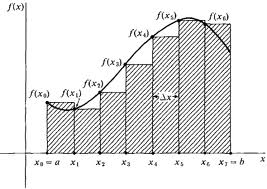
\includegraphics[height=4cm]{area.png}

Fakat bu tur bir anlatim bazen karisikliga yol acabiliyor. Daha iyi bir
anlatim entegralin ``degisen degerlerin carpimi'' oldugudur. Alttaki
resimdeki dikdortgeni dusunelim, 

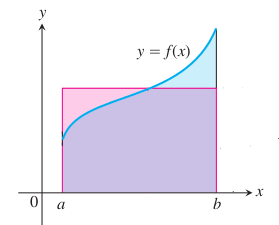
\includegraphics[height=4cm]{box.png}

ve diyelim ki bi dikdortgen, entegralin hesapladigi alani yaklasiksal
olarak temsil ediyor. Dikdortgen alani nasil hesaplanir? Iki kenarinin
carpilmasiyla! Entegral de aslinda boyle bir hesaptir, sadece kenarlardan
biri sabit degildir, ve surekli degismektedir. Bu tur bir anlayis birimleri
sonuca dahil etmek gerektiginde ise yarar, mesela yatay eksen zaman $t$
ise, ve dikey eksen hiz $v(t)$ ise, katedilen mesafe, $v(t)$ nasil bir
sekilde verilmis olursa olsun,

\[ Mesafe = \int v(t)dt \]

formuluyle hesaplanacaktir. Eger hiz ve zaman sabit olsalar, mesela 5 ile 4
gibi, o zaman hesap son derece basit olacakti, 3 x 4 = 12 ile sonucu
bulacaktik. 

Tabii ki carpmak ile toplamak arasinda yakin baglantilar var, mesela 3 x
4'u su sekilde resmedelim

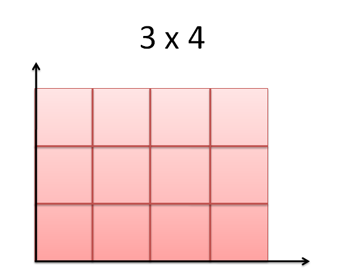
\includegraphics[height=4cm]{grid-multiplication.png}

Burada, evet, 3 degerini dort kere birbiriyle topluyoruz, 3 + 3 + 3 + 3 =
12 ve bu durum 3 x 4 ile ayni sonucu veriyor. Fakat 3'lerin toplami, egri
altindaki alan zihniyetini daha ilerletmeden azicik farkli bir durumu
dusunelim. 

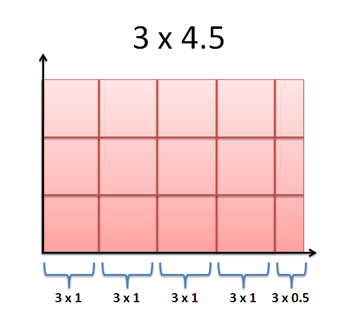
\includegraphics[height=4cm]{piecewise-multiplication.png}

Bu durumda dikey eksendeki kolonlara bir ek yaptik, ama genisligi tam bir
kolon degil, yarim bir kolon ekledik. Bu durumda alan hesabini sadece dikey
kolonlarin toplanmasi olarak yapsakdik 3'u bes kere toplamamiz gerekirdi,
ve yanlis bir hesap yapmis olurduk.

Ilk ornege donersek, diyelim ki $v(t) = 2t$ ve tamam carpim kullanalim,
$t
\cdot 2t$ diyemez miyiz? 

Bu da olmaz, cunku $t\cdot 2t = 2t^2$ bize sadece tek bir $t$ anindaki bir
hesabi veriyor. Biz verilen bir baslangic ve bitis noktalari arasindaki
``tum $t$'ler uzerindeki'' katedilen mesafeyle ilgileniyoruz.  

Yani entegral denince aklimiza carpim gelsin, $x,y$ eksenleri baglaminda,
$y$ eksenindeki $f(x)$'i $x$'i carpiyoruz, bu carpim $x$ icin entegrale
$dx$ olarak yansiyor, $f(x)$ ise entegre edilen fonksiyon haline geliyor. 

Kaynaklar

http://betterexplained.com/articles/a-calculus-analogy-integrals-as-multiplication/

\end{document}
